\section{Experimental Results} \label{sec5}
\noindent
We have built an end-to-end tool in Python for code replacement attack detection.
The tool takes in a set of control loop descriptions, computes their intersection and 
implements the cycle detection step. The tool has been applied to a number of small 
examples of synthetic control applications and their variants. Due to the lack of standard open
source benchmarks in this domain, we have performed all our experiments on synthetic benchmarks of various representative sizes, varying the number of individual control loops, and the number of constituent states of each. For each row, for a fixed number of automatons, we took up the initial descriptions and created random variants of the modified counterparts, and carried out our analysis. As expected, our tool was able to flag out the schedulability violation in each of the cases. Table~\ref{table:nonlin} presents the details of our experiments. Column 2 mentions the number of control applications, while the next presents the number of states in the intersection automaton. Column 4 shows the number of states in the cycle. The final column presents the total time required by our tool for analyzing the schedulability violation in seconds.

\begin{table}[ht]
\caption{Results}
\centering
\begin{tabular}{|c | c | c | c | c |}
%\hline
\hline %inserts double horizontal lines
Case & No. of           &  No. of states in   & No. of      & Total time taken          \\       
     & of               &  the intersection   & states in   & for scheduling            \\  
     & Statemachines    &  automata           & the cycle   & analysis in seconds   \\
\hline
\hline
1 & 2 & 8 & 6 & 0.00192\\

1 & 2  & 33 & 12 &  0.00106 \\

3 & 3  & 67 & 15 & 0.00584 \\

4 & 3 & 149 & 22 & 0.00654 \\

5 & 5 & 354 & 33 & 0.02401 \\

6 & 5 & 1285 & 128 & 0.37886\\

7 & 8 & 1876 & 302 & 11.30161\\

8 & 12 & 2373 & 189 & 20.39397\\

9 & 16 & 535 & 193 & 49.27363\\

10 & 20 & 290 & 135 & 48.22830\\

\hline

\end{tabular}
\label{table:nonlin}

\end{table}

\begin{comment}
\noindent
We explain our problem statement with a small example. Fig\ref{state} presents three automatons $P,Q$ and $R$ representing three different control applications.
Each has one initial state and an acceptance state. The acceptance states are the bus accessing states
of the automaton. To check for schedulability, we first construct the concurrent composition (the intersection automaton) of the individual automatons, as shown in Fig \ref{state-transition1}. The product construction is a little different from the classical product of finite automatons, and will be explained in the following section. \\ 

\noindent
We now consider a code replacement attack take places on this system. The resulting automaton is depicted in Fig \ref{replaced}.
As a result of this attack, one of the control loops is changed, as a result of which, there is a change in the structure of the intersection automaton. Our schedulability assessment on the new product automaton fails. As we can see in Fig \ref{graph_replaced}, there are no cycles which satisfy our infinitary scheduling condition, thus schedulability is no longer guaranteed and we conclude that a code replacement attack has taken place.

\begin{figure}
\begin{center}
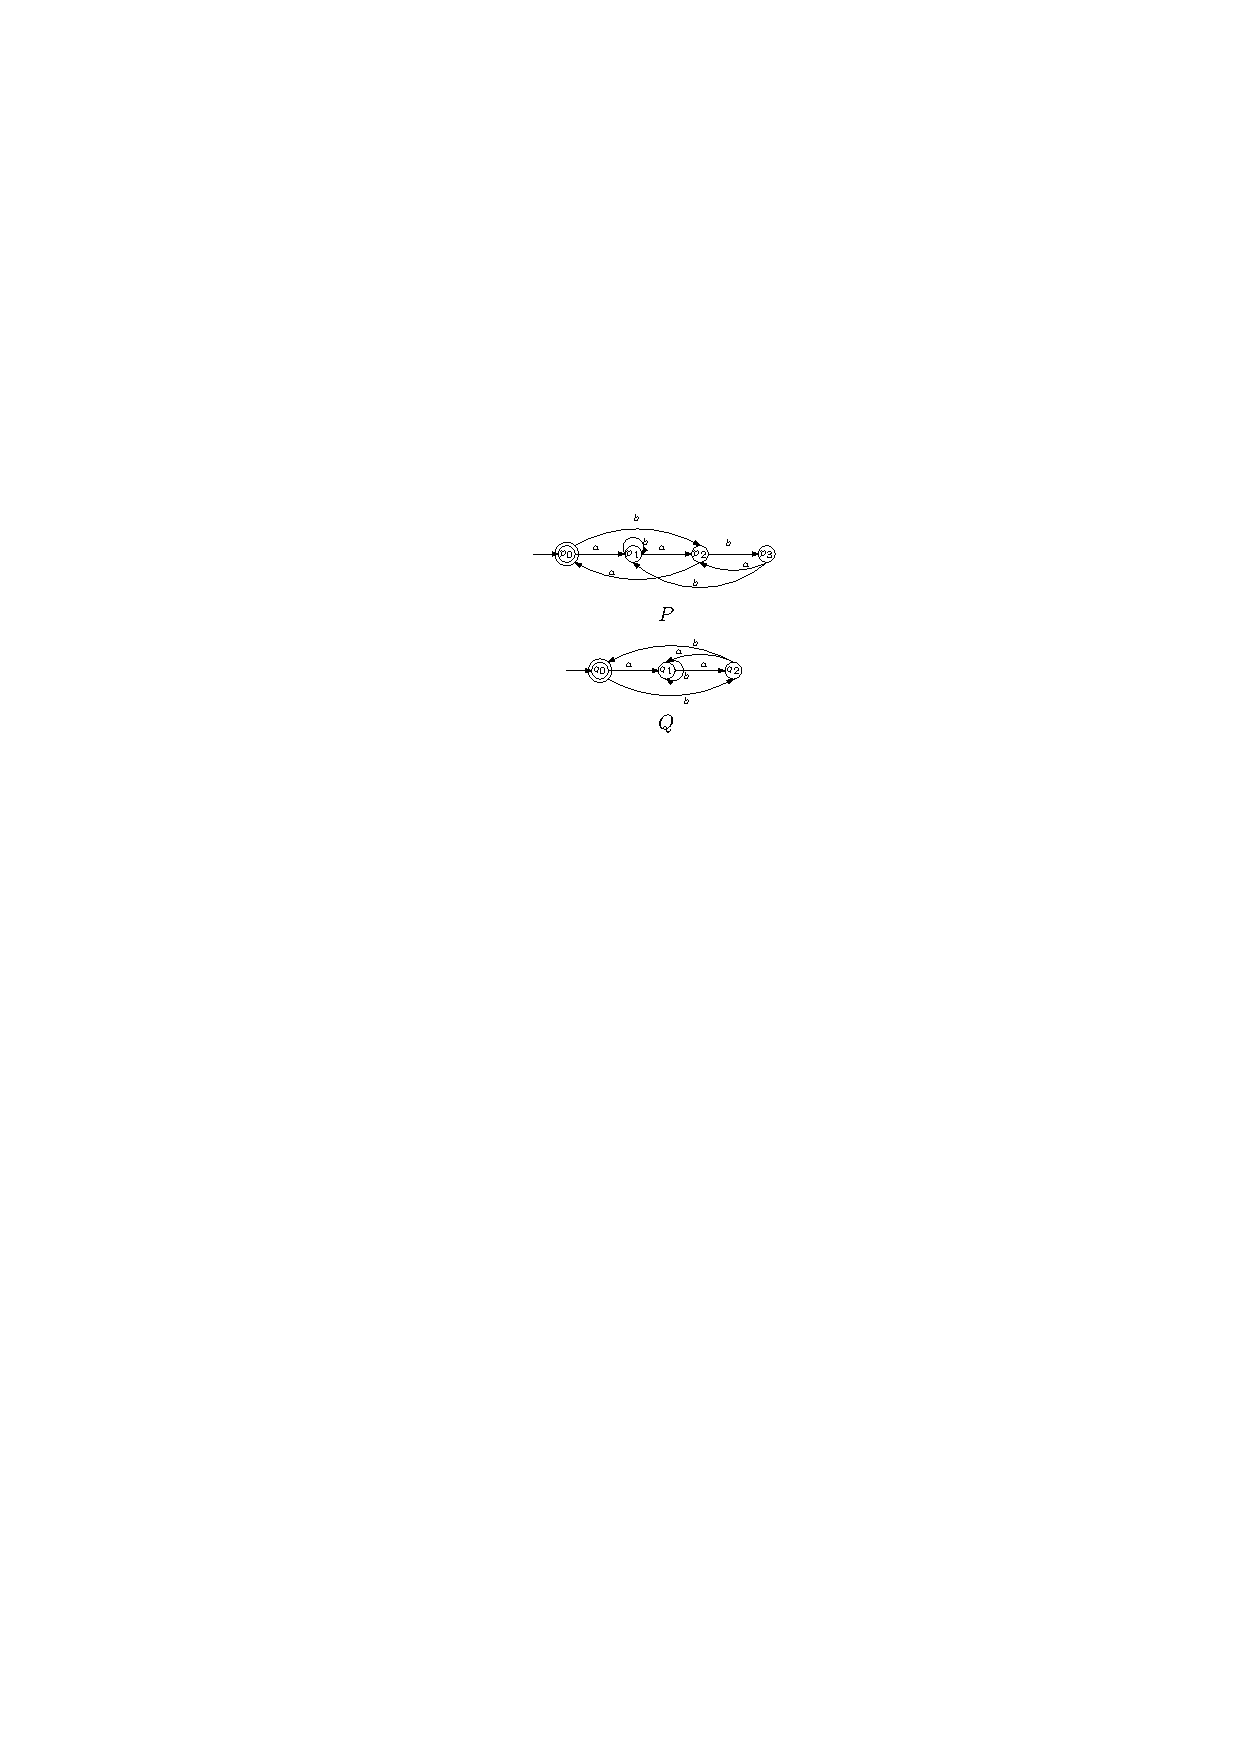
\includegraphics[width=50mm]{motivating_example_automata.pdf}
\end{center}
\vspace{-0.1in}
\caption{{\em Initial Control loops}}
\label{state}
\end{figure}

\begin{figure}
\begin{center}
\includegraphics[width= 75mm]{graph.eps}
\end{center}
%\vspace{-0.1in}
\caption{{\em Initial Intersection automaton}}
\label{state-transition1}
\end{figure}

\begin{figure}
\begin{center}
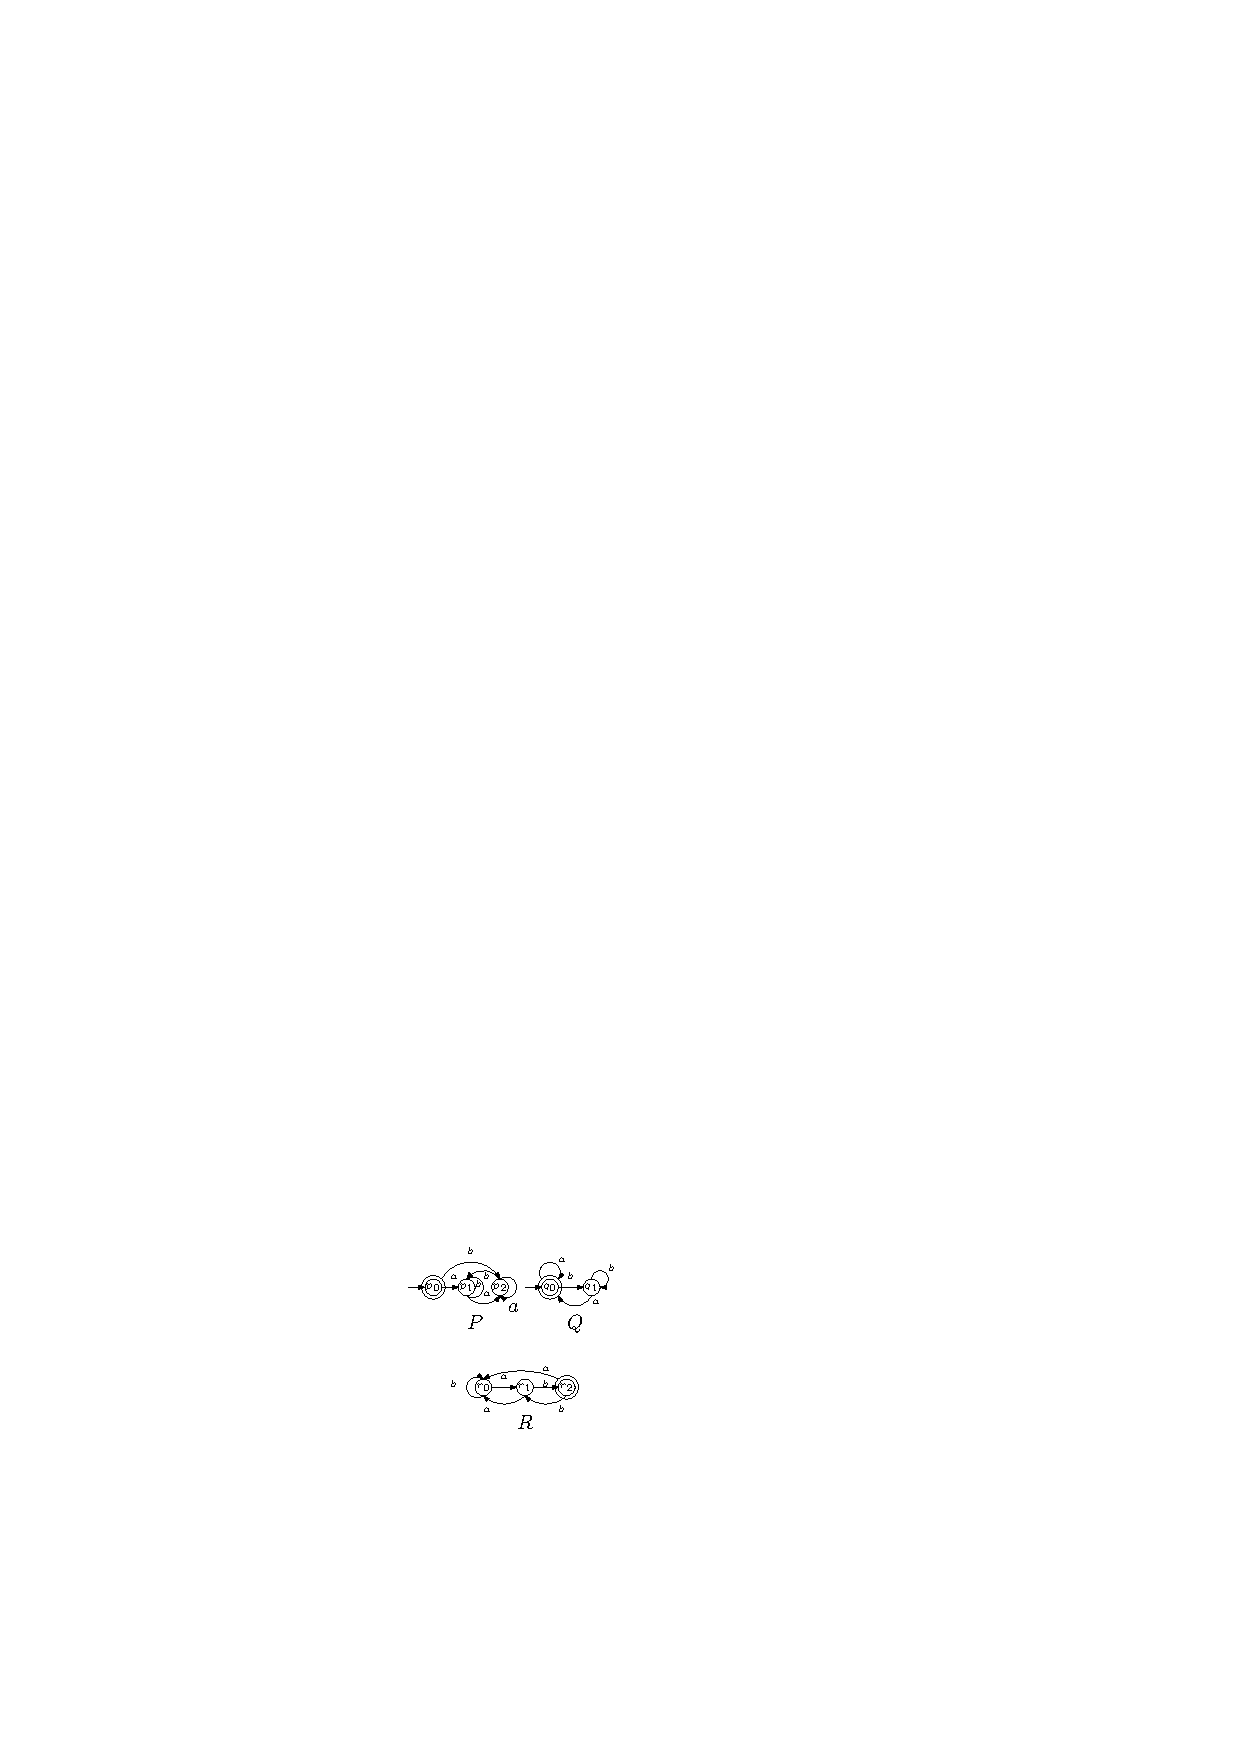
\includegraphics[width= 50mm]{replaced.pdf}
\end{center}
%\vspace{-0.1in}
\caption{{\em Modified control loops after a replacement attack}}
\label{replaced}
\end{figure}


\begin{figure}
\begin{center}
\includegraphics[width= 50mm]{graph_replaced.eps}
\end{center}
%\vspace{-0.1in}
\caption{{\em Intersection automaton after a code replacement attack}}
\label{graph_replaced}
\end{figure}
\end{comment}